\documentclass[12pt]{article}\usepackage[]{graphicx}\usepackage[]{color}
% maxwidth is the original width if it is less than linewidth
% otherwise use linewidth (to make sure the graphics do not exceed the margin)
\makeatletter
\def\maxwidth{ %
  \ifdim\Gin@nat@width>\linewidth
    \linewidth
  \else
    \Gin@nat@width
  \fi
}
\makeatother

\definecolor{fgcolor}{rgb}{0, 0, 0}
\newcommand{\hlnum}[1]{\textcolor[rgb]{0.69,0.494,0}{#1}}%
\newcommand{\hlstr}[1]{\textcolor[rgb]{0.749,0.012,0.012}{#1}}%
\newcommand{\hlcom}[1]{\textcolor[rgb]{0.514,0.506,0.514}{\textit{#1}}}%
\newcommand{\hlopt}[1]{\textcolor[rgb]{0,0,0}{#1}}%
\newcommand{\hlstd}[1]{\textcolor[rgb]{0,0,0}{#1}}%
\newcommand{\hlkwa}[1]{\textcolor[rgb]{0,0,0}{\textbf{#1}}}%
\newcommand{\hlkwb}[1]{\textcolor[rgb]{0,0.341,0.682}{#1}}%
\newcommand{\hlkwc}[1]{\textcolor[rgb]{0,0,0}{\textbf{#1}}}%
\newcommand{\hlkwd}[1]{\textcolor[rgb]{0.004,0.004,0.506}{#1}}%
\let\hlipl\hlkwb

\usepackage{framed}
\makeatletter
\newenvironment{kframe}{%
 \def\at@end@of@kframe{}%
 \ifinner\ifhmode%
  \def\at@end@of@kframe{\end{minipage}}%
  \begin{minipage}{\columnwidth}%
 \fi\fi%
 \def\FrameCommand##1{\hskip\@totalleftmargin \hskip-\fboxsep
 \colorbox{shadecolor}{##1}\hskip-\fboxsep
     % There is no \\@totalrightmargin, so:
     \hskip-\linewidth \hskip-\@totalleftmargin \hskip\columnwidth}%
 \MakeFramed {\advance\hsize-\width
   \@totalleftmargin\z@ \linewidth\hsize
   \@setminipage}}%
 {\par\unskip\endMakeFramed%
 \at@end@of@kframe}
\makeatother

\definecolor{shadecolor}{rgb}{.97, .97, .97}
\definecolor{messagecolor}{rgb}{0, 0, 0}
\definecolor{warningcolor}{rgb}{1, 0, 1}
\definecolor{errorcolor}{rgb}{1, 0, 0}
\newenvironment{knitrout}{}{} % an empty environment to be redefined in TeX

\usepackage{alltt}

\usepackage[hmargin=1in,vmargin=1in]{geometry}
\usepackage{parskip}
\usepackage[hidelinks]{hyperref}
%\hypersetup{pdfstartview=FitV,hidelinks}




%% knitr stuff
%% New command for inline code that isn't to be evaluated

\definecolor{inlinecolor}{rgb}{0.878, 0.918, 0.933}         % edit-kwrite
\newcommand{\inr}[1]{\colorbox{inlinecolor}{\texttt{#1}}}
\IfFileExists{upquote.sty}{\usepackage{upquote}}{}
\begin{document}

{
  \Large
  \centering
  {\bf Lab 10 -- Estimating abundance with
    closed-population capture-mark-recapture data} \\
  Due before your next lab \par
}

\vspace{10pt}


The purpose of this lab is to learn how to estimate abundance using
mark-recapture data from surveys of closed populations. A closed
population does not experience recruitment, mortality, immigration or
emigration. The closure assumption is usually only valid over very
short time periods. We will learn how to work with data from open
populations later.

Work through the problems below, put your answers in a Word file,
and then upload it to ELC. Name the file something like
``Chandler-lab10.docx''.  




%\clearpage

\section*{\large Part I: Lincoln-Peterson estimation}
Suppose you capture, mark, and release 100 largmouth bass ({\it
  Micropterus salmoides}) at Lake Herrick. The next day, you return
and capture 50 individuals, 25 of which were marked on the first
occasion. What is the Lincoln-Peterson estimate of abundance ($N$)?
You do not need to use MARK or R for this -- you can do it by
hand. Be sure to show your work.  

% \begin{figure}[h!]
%   \centering
%   \fbox{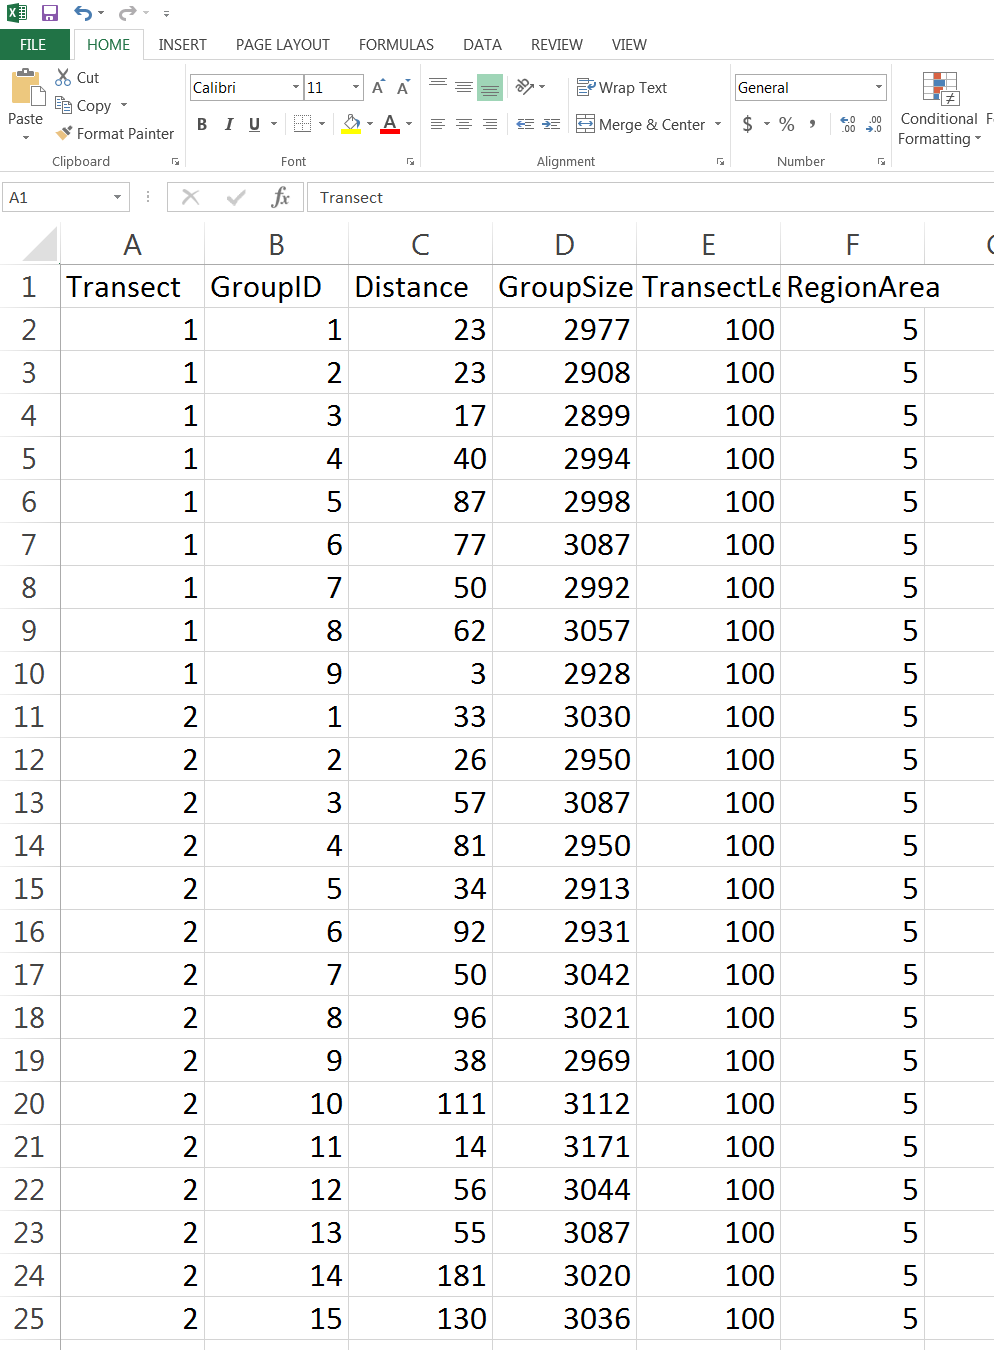
\includegraphics[height=8.5cm]{figs/ds-data1}} \hfill
%   \fbox{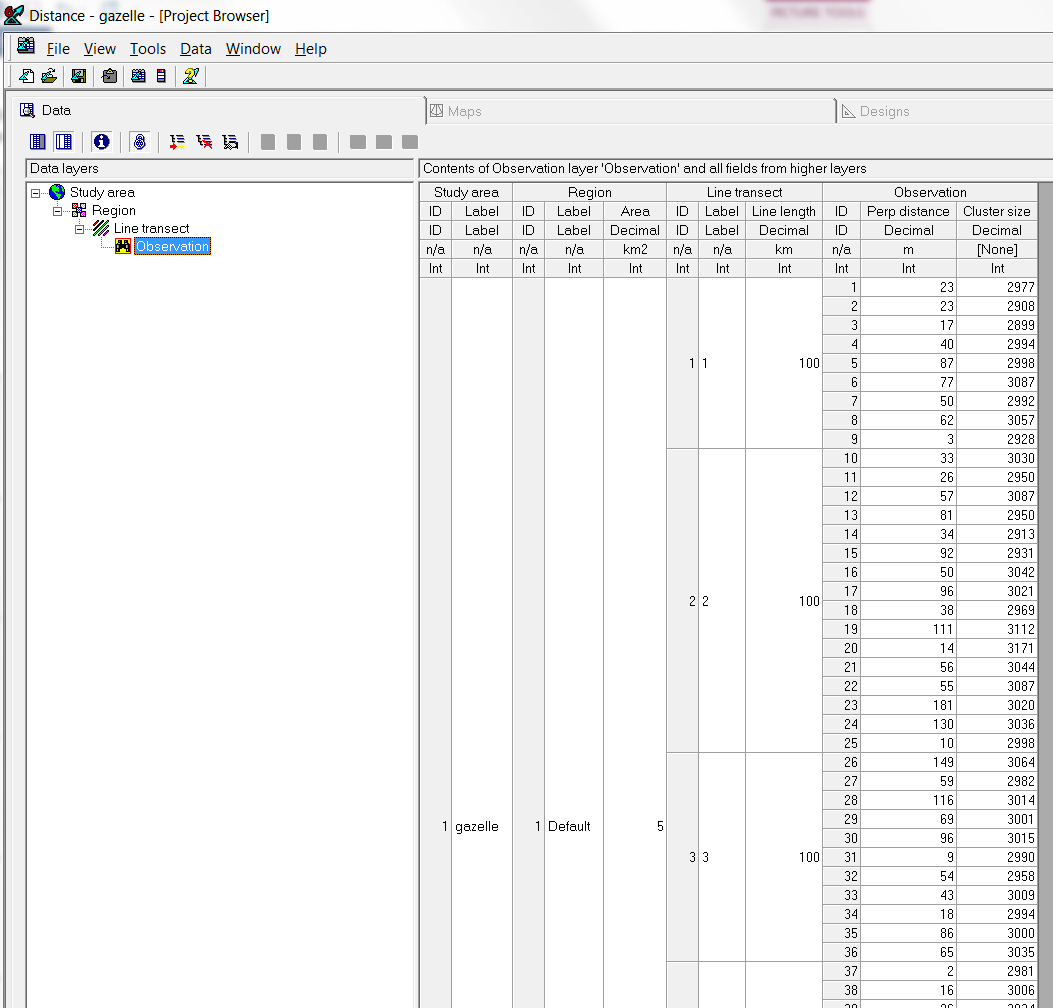
\includegraphics[height=8.5cm]{figs/ds-data2}}   \\
%   \caption{\small Data formatted in Excel (left) and the same data in
%     program DISTANCE.}
%   \label{fig:ds-data}
% \end{figure}
%\clearpage



%\clearpage

\section*{\large  Part II: Closed-population models in MARK and R}

You will use either program MARK or R to fit the four mark-recapture
models described in Table~\ref{tab:Otis}. Undergrads with access to
Windows can use program MARK. Everyone else can use the R package
`mra'. Software instructions are below. The assignment is at the end.  

\begin{table}[h!]
  \centering
  \caption{A description of the four models to be fitted to the
    stinkpot data.}
  \footnotesize
  \begin{tabular}[h!]{ll}
    \hline
    Model & Description \\
    \hline
    $M_0$ & The most basic model in which $p$ and $c$ are constant \\
    $M_t$ & $p$ differs among sampling occasions and $p_t=c_t$. \\
    $M_b$ & Behavioral response model in which $p$ and $c$
            differ. Can describe trap happiness or trap shiness. \\
    $M_{tb}$ & A combination of models $M_t$ and $M_b$. \\
    \hline
  \end{tabular}
  \label{tab:Otis}
\end{table}


%\clearpage

% \begin{figure}[h!]
%   \centering
%   \fbox{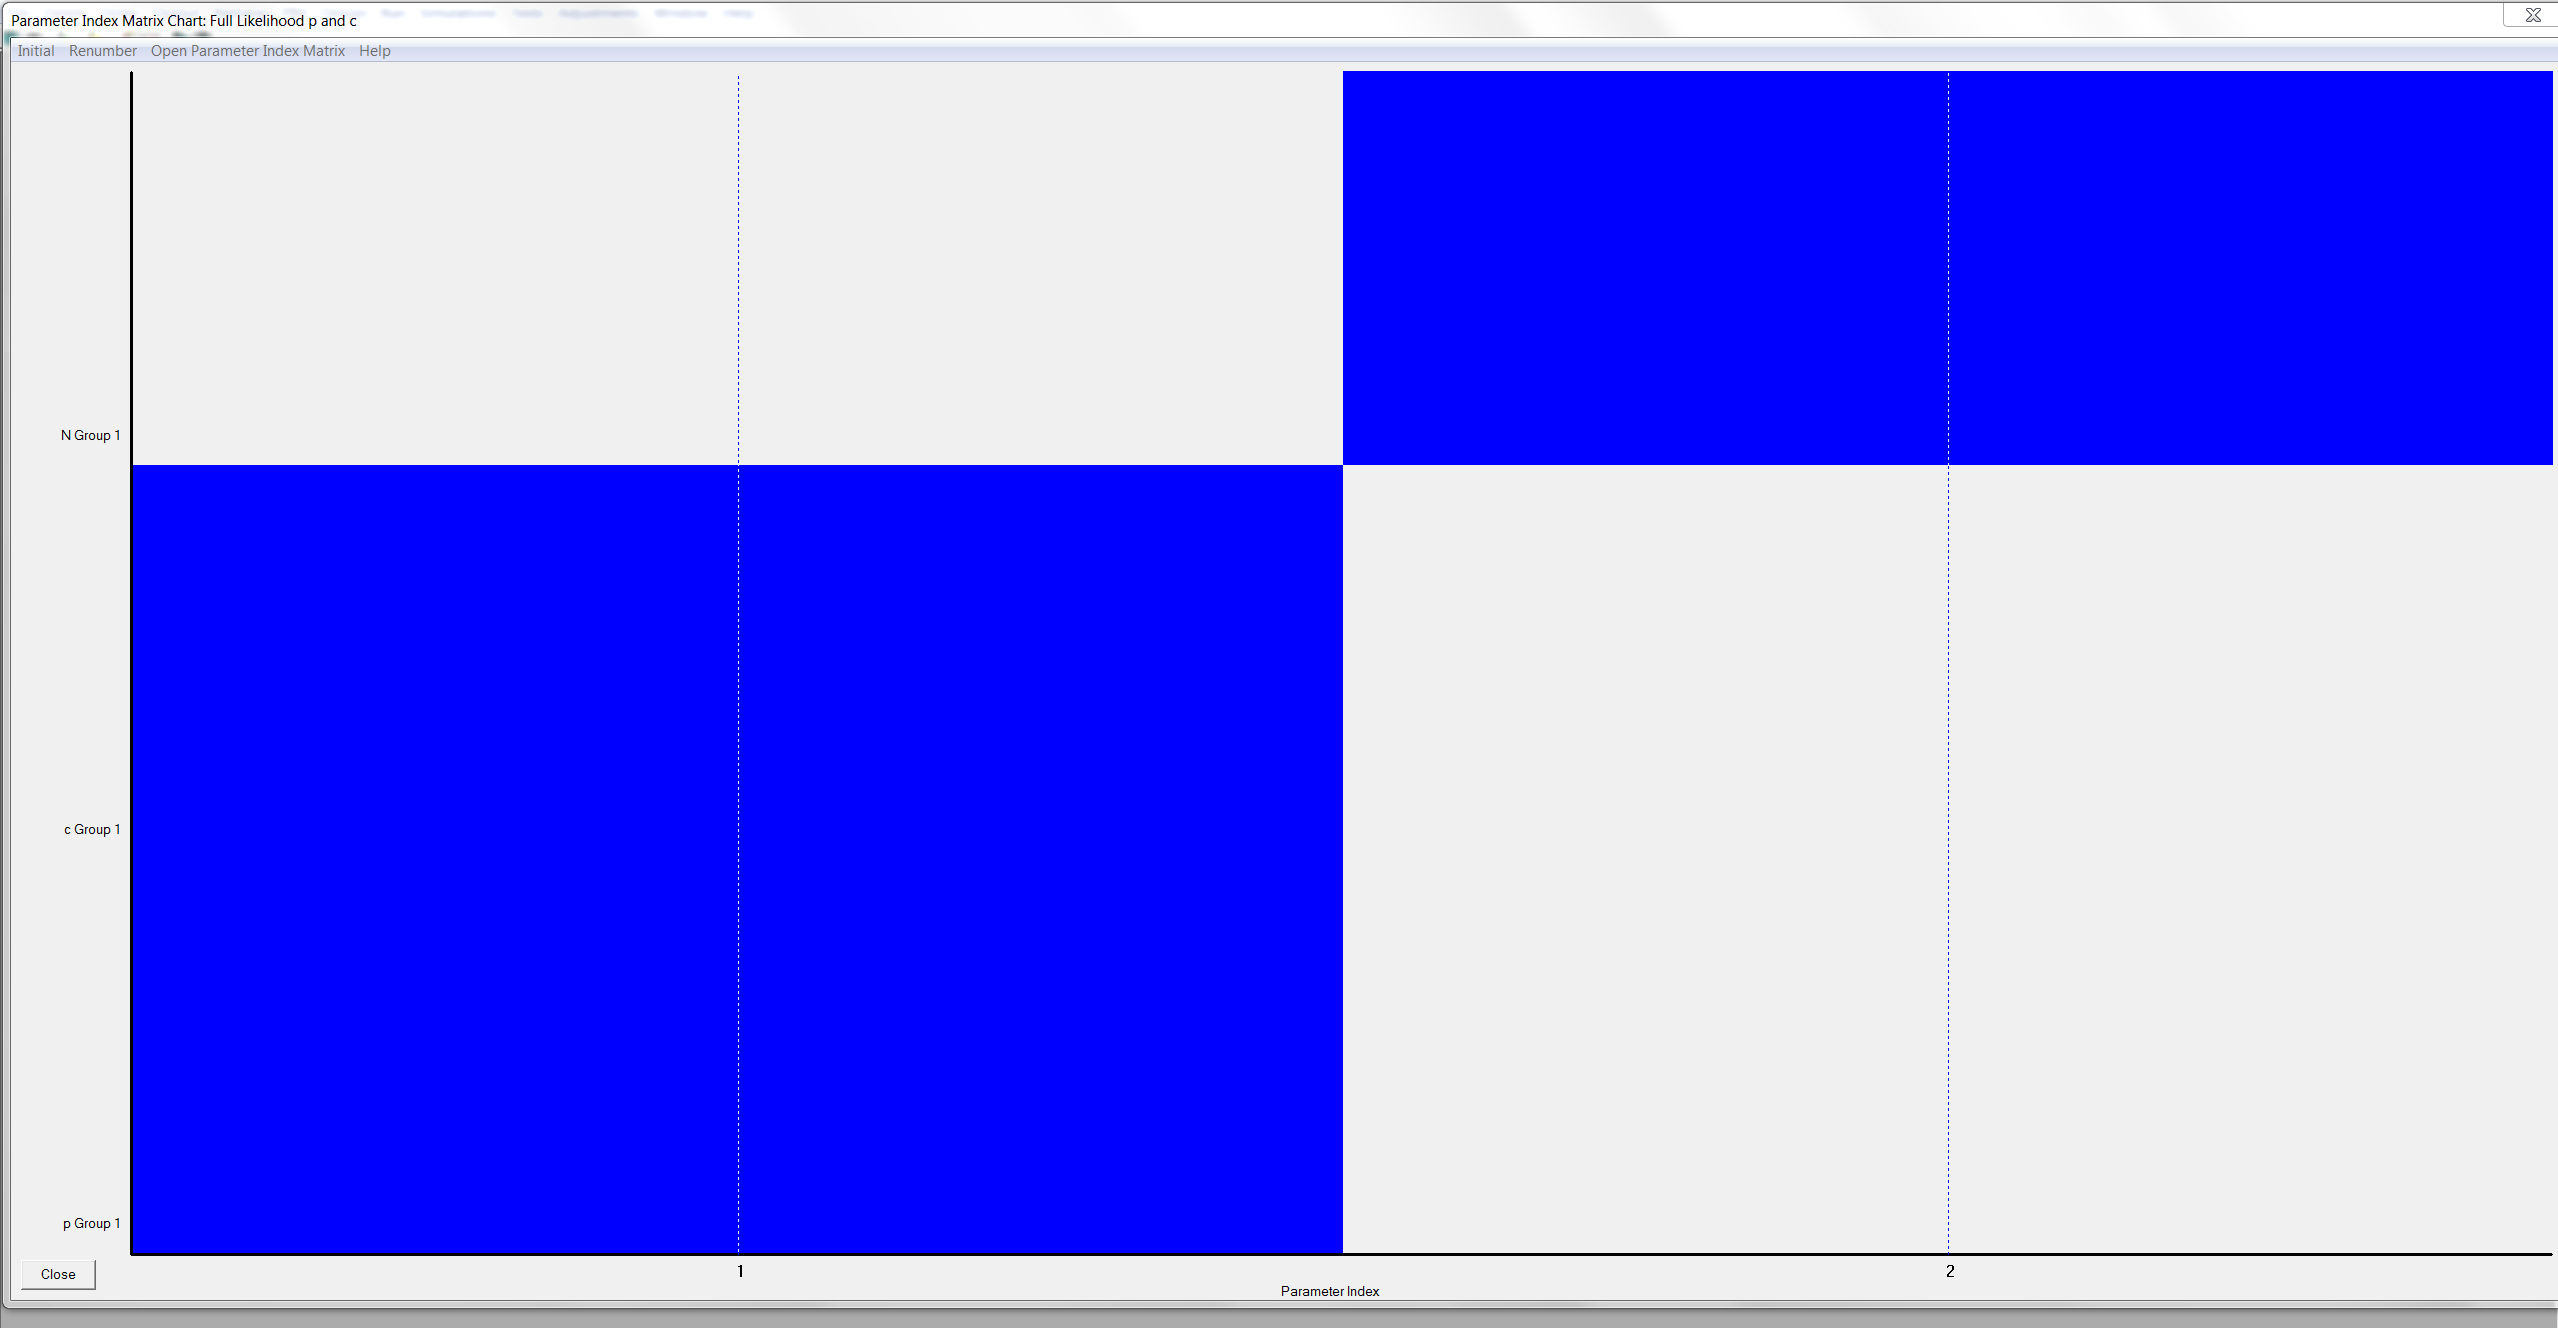
\includegraphics[width=0.9\textwidth]{figs/pim-chart}}
%   \caption{\small The parameter index chart in MARK can be
%     used to specify models. In this case, capture probability ($p$) is
%     set to be equal to recapture probability ($c$).}
%   \label{fig:pim}
% \end{figure}

% \vspace{1cm}

{\bf Parameter definitions}
\begin{itemize}
  \item $p$ -- capture probability. The probability of capturing an
    individual on a single occasion
  \item $p_t$ -- capture probability on occasion $t$
  \item $c$ -- recapture probability. The probability of capturing an
    individual that has been captured previously.
  \item $n$ -- the number of individuals captured
  \item $f_0$ -- the number of individual not captured
  \item $N$ -- abundance. The number of individuals in the
    population. $N=n+f_0$. 
\end{itemize}

%\vspace{1cm}



\subsection*{Closed-population models in program MARK}

You can download program MARK here:
\url{http://www.phidot.org/software/mark/downloads/}. Even though it
is possible to run MARK on Linux or OS/X, it isn't easy, and I don't
recommend it. If you don't have Windows, use R as described below.

The data file (\verb+CH-SO-Andy07.inp+) is a simple text file, formatted
as required by program MARK. Each row of the file is a capture history
for each of the 17 stinkpots ({\it Sternotherus odoratus}) captured in
2007 (May 31 - June 5). There were 6 capture occasions, so for every
turtle, there are 6 ones and zeros indicating if the turtle was
captured on that occasion or not. After each capture history is a
space followed by a 1 and a semi-colon to indicate that there was just
1 turtle with this history (Fig.~\ref{fig:stink07-data}).

\begin{figure}[h!]
  \centering
  \fbox{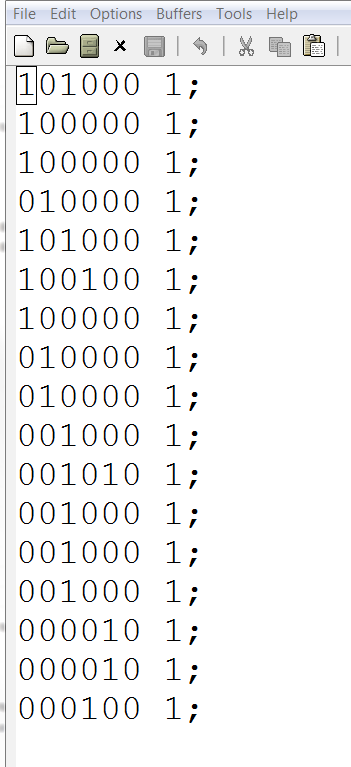
\includegraphics[height=0.6\textheight]{figs/stinkpot07-data}}
  \caption{\small Stinkpot capture histories in a text file ready to
    be imported to MARK.}
  \label{fig:stink07-data}
\end{figure}

\clearpage

{\bf Instructions}
\begin{enumerate}
  \item[(i)] Open MARK and create a new project by selecting:
    \verb+"File > New"+.
  \item[(ii)] Name the project ``Exercise I'' and select the encounter
    history file \verb+"CH-SO-Andy07.inp"+ (see
    Fig.~\ref{fig:stink07-data})
  \item[(iii)] Choose \verb+"Closed Captures"+ from the list of ``data
    types'' on the left and then select %\verb+"Full likelihood p and c"+.
    \verb+"Huggins' p and c"+.
  \item[(iv)] Set the number of encounter occasions to 6, then hit
    \verb+"OK"+
\end{enumerate}

\begin{figure}[h!]
  \centering
  \fbox{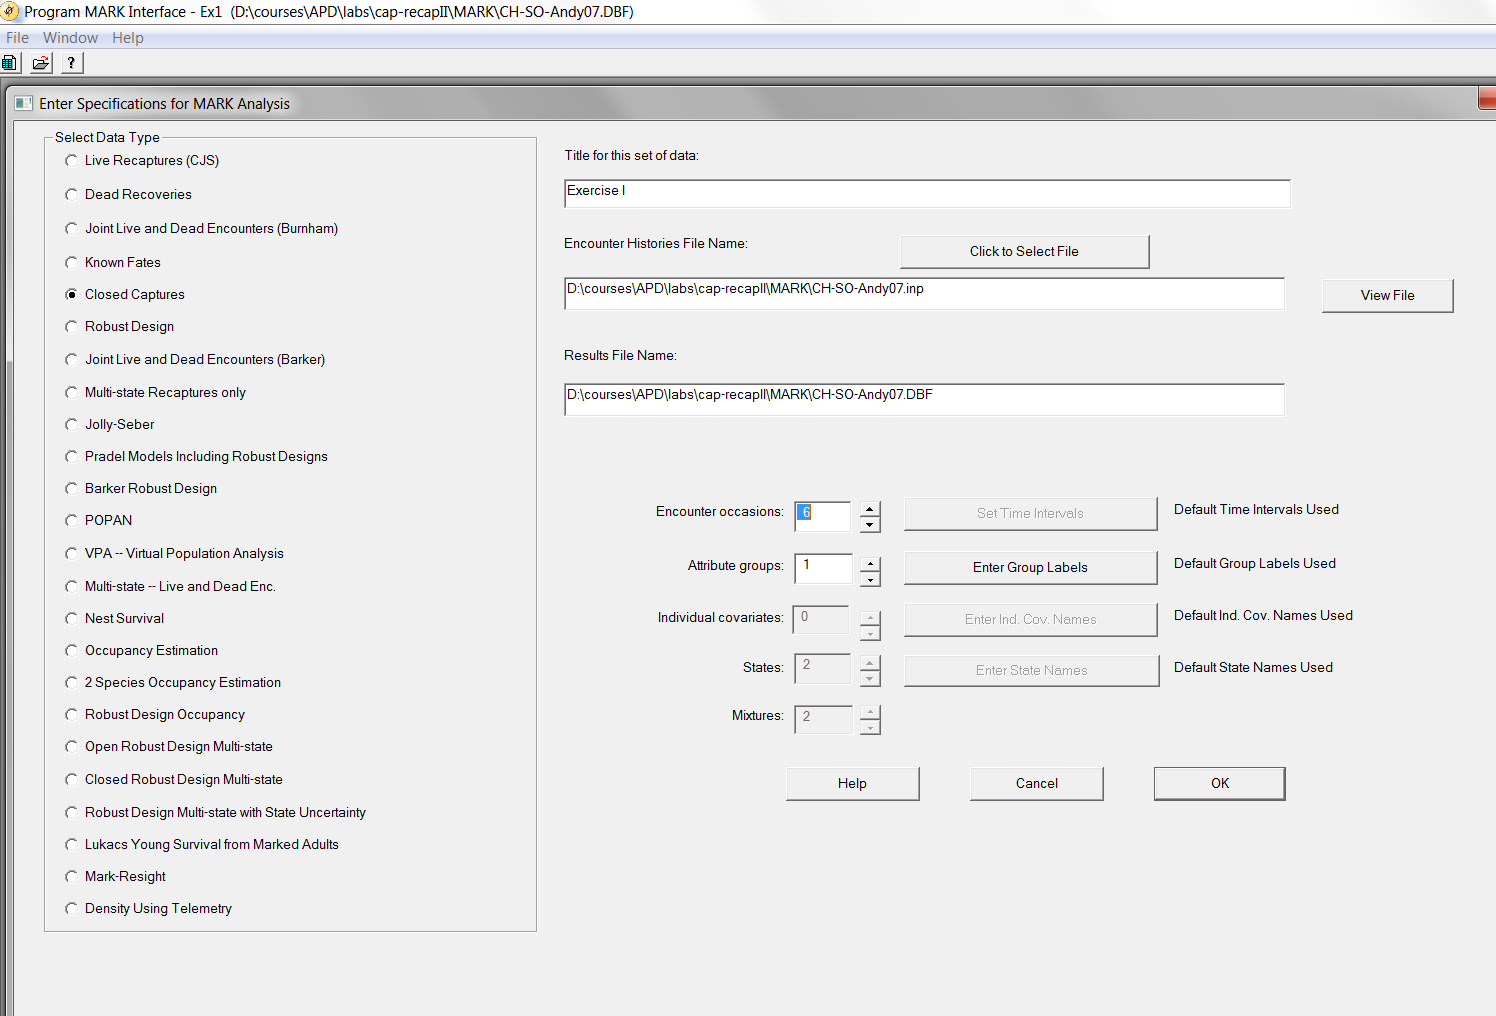
\includegraphics[width=0.8\textwidth]{figs/stinkpot07-MARK}}
  \caption{\small Setting up the MARK analysis of the stinkpot data.}
  \label{fig:stink07-mark}
\end{figure}

\begin{enumerate}
  \item[(v)] Run four models differing in their specifications of
    capture probability ($p$) and recapture probability ($c$) by
    clicking on  \verb+"Run > Pre-defined Model(s)"+. Next, click on the
    \verb+"Select Models"+ button and choose models \verb+"M0"+,
    \verb+"Mt"+, \verb+"Mb"+, and \verb+"Mtb"+. An explanation of these
    models is shown below in Table 1. Next, click \verb+"OK"+, then
    hit \verb+"OK to Run"+. 
  \item[(vi)] Inspect the model results, by right-clicking on one of
    the models in the Results Browser and look at
    \verb+"Real Estimates"+ and \verb+"Derived estimates"+. See
    Table~\ref{tab:Otis} and the parameter definitions above for help
    interpreting ther results.
  % \item[(vii)]	Now, run two more pre-defined models: one with
  %   time-specific capture probabilities \verb+"p(t)"+ and one with
  %   time-specific recapture probabilities \verb+"c(t)"+. These two models can
  %   be run using the same steps above but by choosing \verb+"(t)"+ instead
  %   of \verb+"(.)"+.
  % \item[(viii)] Run a custom model in which capture probability ($p$)
  %   is equal to recapture probability ($c$). You can do this by
  %   selecting \verb+"PIM > Parameter Index Chart"+. Then drag the blue
  %   box for $c$ to the left, so that it is on top of the blue box for $p$
  %   (see Fig.~\ref{fig:pim}). Then select \verb+"Run > Current Model"+.
\end{enumerate}



\clearpage


\section*{Closed-population models in R}


Graduate students and undergraduates without access to Windows, should
follow these instructions (instead of the MARK instructions above) for
completing the assignment. 

Open R (or RStudio) and install the ``mra'' package using the
following command: 

\begin{knitrout}
\definecolor{shadecolor}{rgb}{0.878, 0.918, 0.933}\color{fgcolor}\begin{kframe}
\begin{alltt}
\hlkwd{install.packages}\hlstd{(}\hlstr{"mra"}\hlstd{)}
\end{alltt}
\end{kframe}
\end{knitrout}

Now load the package like so: 

\begin{knitrout}
\definecolor{shadecolor}{rgb}{0.878, 0.918, 0.933}\color{fgcolor}\begin{kframe}
\begin{alltt}
\hlkwd{library}\hlstd{(mra)}
\end{alltt}


{\ttfamily\noindent\itshape\color{messagecolor}{\#\# mra (version 2.16.11)}}\end{kframe}
\end{knitrout}

We can import the data using \inr{read.table}. The only trick is to
tell R that the capture histories should be treated as a character
string, rather than as a numeric variable. The \inr{colClasses}
arguments let's us do that.

\begin{knitrout}
\definecolor{shadecolor}{rgb}{0.878, 0.918, 0.933}\color{fgcolor}\begin{kframe}
\begin{alltt}
\hlstd{capture.histories} \hlkwb{<-} \hlkwd{read.table}\hlstd{(}\hlstr{"CH-SO-Andy07.inp"}\hlstd{,} \hlkwc{sep}\hlstd{=}\hlstr{" "}\hlstd{,}
                                \hlkwc{colClasses}\hlstd{=}\hlkwd{c}\hlstd{(}\hlstr{"character"}\hlstd{,} \hlstr{"character"}\hlstd{),}
                                \hlkwc{col.names}\hlstd{=}\hlkwd{c}\hlstd{(}\hlstr{"ch"}\hlstd{,} \hlstr{"freq"}\hlstd{))}
\end{alltt}
\end{kframe}
\end{knitrout}

It's a small dataset, so we can display it in full:

\begin{knitrout}
\definecolor{shadecolor}{rgb}{0.878, 0.918, 0.933}\color{fgcolor}\begin{kframe}
\begin{alltt}
\hlstd{capture.histories}
\end{alltt}
\begin{verbatim}
##        ch freq
## 1  101000   1;
## 2  100000   1;
## 3  100000   1;
## 4  010000   1;
## 5  101000   1;
## 6  100100   1;
## 7  100000   1;
## 8  010000   1;
## 9  010000   1;
## 10 001000   1;
## 11 001010   1;
## 12 001000   1;
## 13 001000   1;
## 14 001000   1;
## 15 000010   1;
## 16 000010   1;
## 17 000100   1;
\end{verbatim}
\end{kframe}
\end{knitrout}

% As you can see, no turtle was caught more than twice out of the 6
% occassions.

% Run this command to convert this to format that \inr{secr} recognizes:

% <<format>>=
% cap.hist <- unRMarkInput(capture.histories, covariates=FALSE)
% @ 


% <<closedN>>=
% closedN(cap.hist, estimator=c("null", "darroch", "zippin"))
% @ 


% <<Rcapture>>=
% library(Rcapture)
% closedp(cap.hist[,,1])
% @ 

We need to convert the capture histories from a character vector to a
matrix. The following code does the trick.


\begin{knitrout}
\definecolor{shadecolor}{rgb}{0.878, 0.918, 0.933}\color{fgcolor}\begin{kframe}
\begin{alltt}
\hlstd{ch.mat} \hlkwb{<-} \hlkwd{t}\hlstd{(}\hlkwd{sapply}\hlstd{(capture.histories}\hlopt{$}\hlstd{ch,}
                   \hlkwa{function}\hlstd{(}\hlkwc{x}\hlstd{)} \hlkwd{as.integer}\hlstd{(}\hlkwd{strsplit}\hlstd{(x,} \hlstr{""}\hlstd{)[[}\hlnum{1}\hlstd{]])))}
\hlkwd{dimnames}\hlstd{(ch.mat)} \hlkwb{<-} \hlkwd{list}\hlstd{(}\hlkwd{paste0}\hlstd{(}\hlstr{"Turtle"}\hlstd{,} \hlnum{1}\hlopt{:}\hlnum{17}\hlstd{),} \hlkwd{paste0}\hlstd{(}\hlstr{"Time"}\hlstd{,} \hlnum{1}\hlopt{:}\hlnum{6}\hlstd{))}
\end{alltt}
\end{kframe}
\end{knitrout}


Now the capture histories look like this:

\begin{knitrout}
\definecolor{shadecolor}{rgb}{0.878, 0.918, 0.933}\color{fgcolor}\begin{kframe}
\begin{alltt}
\hlstd{ch.mat}
\end{alltt}
\begin{verbatim}
##          Time1 Time2 Time3 Time4 Time5 Time6
## Turtle1      1     0     1     0     0     0
## Turtle2      1     0     0     0     0     0
## Turtle3      1     0     0     0     0     0
## Turtle4      0     1     0     0     0     0
## Turtle5      1     0     1     0     0     0
## Turtle6      1     0     0     1     0     0
## Turtle7      1     0     0     0     0     0
## Turtle8      0     1     0     0     0     0
## Turtle9      0     1     0     0     0     0
## Turtle10     0     0     1     0     0     0
## Turtle11     0     0     1     0     1     0
## Turtle12     0     0     1     0     0     0
## Turtle13     0     0     1     0     0     0
## Turtle14     0     0     1     0     0     0
## Turtle15     0     0     0     0     1     0
## Turtle16     0     0     0     0     1     0
## Turtle17     0     0     0     1     0     0
\end{verbatim}
\end{kframe}
\end{knitrout}

We will use the \inr{F.huggins.estim} function to fit the
closed population models. Model $M_0$ can be fit like this: 

\begin{knitrout}
\definecolor{shadecolor}{rgb}{0.878, 0.918, 0.933}\color{fgcolor}\begin{kframe}
\begin{alltt}
\hlstd{M0} \hlkwb{<-} \hlkwd{F.huggins.estim}\hlstd{(}\hlkwc{capture}\hlstd{=}\hlopt{~}\hlnum{1}\hlstd{,} \hlkwc{recapture}\hlstd{=}\hlkwa{NULL}\hlstd{,} \hlkwc{histories}\hlstd{=ch.mat)}
\end{alltt}
\end{kframe}
\end{knitrout}

Model $M_b$ like this:

\begin{knitrout}
\definecolor{shadecolor}{rgb}{0.878, 0.918, 0.933}\color{fgcolor}\begin{kframe}
\begin{alltt}
\hlstd{Mb} \hlkwb{<-} \hlkwd{F.huggins.estim}\hlstd{(}\hlkwc{capture}\hlstd{=}\hlopt{~}\hlnum{1}\hlstd{,} \hlkwc{recapture}\hlstd{=}\hlopt{~}\hlnum{1}\hlstd{,} \hlkwc{histories}\hlstd{=ch.mat)}
\end{alltt}
\end{kframe}
\end{knitrout}

To fit model $M_t$, we have to create a time variable.

\begin{knitrout}
\definecolor{shadecolor}{rgb}{0.878, 0.918, 0.933}\color{fgcolor}\begin{kframe}
\begin{alltt}
\hlstd{time} \hlkwb{<-} \hlkwd{tvar}\hlstd{(}\hlkwd{factor}\hlstd{(}\hlnum{1}\hlopt{:}\hlnum{6}\hlstd{),} \hlkwc{nan}\hlstd{=}\hlnum{17}\hlstd{)} \hlcom{## 6 time periods. 17 animals.}
\hlstd{Mt} \hlkwb{<-} \hlkwd{F.huggins.estim}\hlstd{(}\hlkwc{capture}\hlstd{=}\hlopt{~}\hlstd{time,} \hlkwc{recapture}\hlstd{=}\hlkwa{NULL}\hlstd{,} \hlkwc{histories}\hlstd{=ch.mat)}
\end{alltt}
\end{kframe}
\end{knitrout}


You should be able to figure out how to fit model $M_{tb}$ by
extending the code above.

Estimates of abundance along with AICc values can be found by typing
the name of the fitted model object. For example:

\begin{knitrout}
\definecolor{shadecolor}{rgb}{0.878, 0.918, 0.933}\color{fgcolor}\begin{kframe}
\begin{alltt}
\hlstd{M0}
\end{alltt}
\begin{verbatim}
## Call:
## F.huggins.estim(capture = ~1, recapture = NULL, histories = ch.mat)
## 
##  Capture and Recapture model:
##  Variable     Est       SE     
##  (Intercept)  -2.37255  0.49911 
## 
## Population Size Estimate (se): 41.0364 (16.6626)
## 95% confidence interval for population size: 24.04 to 99.05
## Individuals observed: 17
## Effective sample size: 102
## 
## Message =  SUCCESS: Convergence criterion met
## Number of estimable coefficients (estimated) =  1
## Log likelihood =  -43.9354578026216
## Deviance =  87.8709156052432
## AIC =  89.8709156052432
## AICc =  89.9109156052432
\end{verbatim}
\end{kframe}
\end{knitrout}


You can extract information about capture probability (which isn't
needed to do the assignment) using code like this:

\begin{knitrout}
\definecolor{shadecolor}{rgb}{0.878, 0.918, 0.933}\color{fgcolor}\begin{kframe}
\begin{alltt}
\hlkwd{round}\hlstd{(M0}\hlopt{$}\hlstd{p.hat,} \hlnum{3}\hlstd{)}
\end{alltt}
\begin{verbatim}
##        [,1]  [,2]  [,3]  [,4]  [,5]  [,6]
##  [1,] 0.085 0.085 0.085 0.085 0.085 0.085
##  [2,] 0.085 0.085 0.085 0.085 0.085 0.085
##  [3,] 0.085 0.085 0.085 0.085 0.085 0.085
##  [4,] 0.085 0.085 0.085 0.085 0.085 0.085
##  [5,] 0.085 0.085 0.085 0.085 0.085 0.085
##  [6,] 0.085 0.085 0.085 0.085 0.085 0.085
##  [7,] 0.085 0.085 0.085 0.085 0.085 0.085
##  [8,] 0.085 0.085 0.085 0.085 0.085 0.085
##  [9,] 0.085 0.085 0.085 0.085 0.085 0.085
## [10,] 0.085 0.085 0.085 0.085 0.085 0.085
## [11,] 0.085 0.085 0.085 0.085 0.085 0.085
## [12,] 0.085 0.085 0.085 0.085 0.085 0.085
## [13,] 0.085 0.085 0.085 0.085 0.085 0.085
## [14,] 0.085 0.085 0.085 0.085 0.085 0.085
## [15,] 0.085 0.085 0.085 0.085 0.085 0.085
## [16,] 0.085 0.085 0.085 0.085 0.085 0.085
## [17,] 0.085 0.085 0.085 0.085 0.085 0.085
\end{verbatim}
\end{kframe}
\end{knitrout}

For model $M_0$, capture probability is the same for all individuals
during all time periods. This won't be the case for the other models. 

\clearpage

\section*{Assignment}

\begin{enumerate}
  \item[(a)] Summarize your results by creating a table in which each row
    is a model, and include the following columns: the estimates of $N$
    (abundance), the standard errors of $N$ (SE), and the AICc
    values. 
  \item[(b)] The model with the lowest AICc is considered the best in
    the set of models. Which model has the lowest AICc? Do your
    results suggest that it is important to account for variation in
    capture (and recapture) probability over time? Explain.
  \item[(c)] Why do you think model $M_0$ is the worst model
    in the set? Look at the capture histories when answering this
    question. 
  \item[(d)] Given what you know about turtles and turtle trapping,
    what sources of variation in capture probability (other than time)
    do you think we might want to account for to obtain more reliable
    abundance estimates?
\end{enumerate}





\end{document}




